\documentclass{article}\usepackage[]{graphicx}\usepackage[]{xcolor}
% maxwidth is the original width if it is less than linewidth
% otherwise use linewidth (to make sure the graphics do not exceed the margin)
\makeatletter
\def\maxwidth{ %
  \ifdim\Gin@nat@width>\linewidth
    \linewidth
  \else
    \Gin@nat@width
  \fi
}
\makeatother

\definecolor{fgcolor}{rgb}{0.345, 0.345, 0.345}
\newcommand{\hlnum}[1]{\textcolor[rgb]{0.686,0.059,0.569}{#1}}%
\newcommand{\hlsng}[1]{\textcolor[rgb]{0.192,0.494,0.8}{#1}}%
\newcommand{\hlcom}[1]{\textcolor[rgb]{0.678,0.584,0.686}{\textit{#1}}}%
\newcommand{\hlopt}[1]{\textcolor[rgb]{0,0,0}{#1}}%
\newcommand{\hldef}[1]{\textcolor[rgb]{0.345,0.345,0.345}{#1}}%
\newcommand{\hlkwa}[1]{\textcolor[rgb]{0.161,0.373,0.58}{\textbf{#1}}}%
\newcommand{\hlkwb}[1]{\textcolor[rgb]{0.69,0.353,0.396}{#1}}%
\newcommand{\hlkwc}[1]{\textcolor[rgb]{0.333,0.667,0.333}{#1}}%
\newcommand{\hlkwd}[1]{\textcolor[rgb]{0.737,0.353,0.396}{\textbf{#1}}}%
\let\hlipl\hlkwb

\usepackage{framed}
\makeatletter
\newenvironment{kframe}{%
 \def\at@end@of@kframe{}%
 \ifinner\ifhmode%
  \def\at@end@of@kframe{\end{minipage}}%
  \begin{minipage}{\columnwidth}%
 \fi\fi%
 \def\FrameCommand##1{\hskip\@totalleftmargin \hskip-\fboxsep
 \colorbox{shadecolor}{##1}\hskip-\fboxsep
     % There is no \\@totalrightmargin, so:
     \hskip-\linewidth \hskip-\@totalleftmargin \hskip\columnwidth}%
 \MakeFramed {\advance\hsize-\width
   \@totalleftmargin\z@ \linewidth\hsize
   \@setminipage}}%
 {\par\unskip\endMakeFramed%
 \at@end@of@kframe}
\makeatother

\definecolor{shadecolor}{rgb}{.97, .97, .97}
\definecolor{messagecolor}{rgb}{0, 0, 0}
\definecolor{warningcolor}{rgb}{1, 0, 1}
\definecolor{errorcolor}{rgb}{1, 0, 0}
\newenvironment{knitrout}{}{} % an empty environment to be redefined in TeX

\usepackage{alltt}
\usepackage{color}
\usepackage{Sweave}
\IfFileExists{upquote.sty}{\usepackage{upquote}}{}
\begin{document}

\title{HW8}
\author{Charlie Hooey}



Here is my code for the homework 8 assignment, which uses two methods of point estimation in order to see how they line up with a histogram of the provided data's gaussian distribution

\section{R Code and Output}
\begin{knitrout}\scriptsize
\definecolor{shadecolor}{rgb}{0.969, 0.969, 0.969}\color{fgcolor}\begin{kframe}
\begin{alltt}
\hlkwd{suppressPackageStartupMessages}\hldef{(}\hlkwd{library}\hldef{(tidyverse))}
\hlcom{# Load required packages}
\hlkwd{library}\hldef{(ggplot2)}

\hlcom{# Data from Sathar & Jose (2020) / Wilson (1997)}
\hldef{data} \hlkwb{<-} \hlkwd{c}\hldef{(}\hlnum{2944}\hldef{,} \hlnum{3206}\hldef{,} \hlnum{2751}\hldef{,} \hlnum{3089}\hldef{,} \hlnum{3406}\hldef{,} \hlnum{3275}\hldef{,} \hlnum{2606}\hldef{,} \hlnum{2723}\hldef{,} \hlnum{2475}\hldef{,} \hlnum{2930}\hldef{,}
          \hlnum{2530}\hldef{,} \hlnum{2399}\hldef{,} \hlnum{2806}\hldef{,} \hlnum{2827}\hldef{,} \hlnum{2951}\hldef{,} \hlnum{2854}\hldef{,} \hlnum{2930}\hldef{,} \hlnum{2565}\hldef{,} \hlnum{2799}\hldef{,} \hlnum{3102}\hldef{,}
          \hlnum{3454}\hldef{,} \hlnum{4185}\hldef{,} \hlnum{3095}\hldef{,} \hlnum{3247}\hldef{,} \hlnum{3371}\hldef{,} \hlnum{3302}\hldef{,} \hlnum{3544}\hldef{,} \hlnum{3454}\hldef{,} \hlnum{3468}\hldef{,} \hlnum{3233}\hldef{,}
          \hlnum{2571}\hldef{,} \hlnum{3268}\hldef{,} \hlnum{2792}\hldef{,} \hlnum{2916}\hldef{,} \hlnum{3006}\hldef{,} \hlnum{3523}\hldef{,} \hlnum{2958}\hldef{,} \hlnum{3123}\hldef{,} \hlnum{2930}\hldef{,} \hlnum{2689}\hldef{,}
          \hlnum{3075}\hldef{,} \hlnum{3337}\hldef{,} \hlnum{3468}\hldef{,} \hlnum{3254}\hldef{,} \hlnum{3061}\hldef{,} \hlnum{3647}\hldef{,} \hlnum{3295}\hldef{,} \hlnum{2971}\hldef{,} \hlnum{3068}\hldef{,} \hlnum{3371}\hldef{)}

\hlcom{# Number of observations}
\hldef{n} \hlkwb{<-} \hlkwd{length}\hldef{(data)}

\hlcom{# (1) MOM Estimates using sample mean and unbiased sample standard deviation (n-1)}
\hldef{mu_mom} \hlkwb{<-} \hlkwd{mean}\hldef{(data)}
\hldef{sigma_mom} \hlkwb{<-} \hlkwd{sqrt}\hldef{(}\hlkwd{sum}\hldef{((data} \hlopt{-} \hldef{mu_mom)}\hlopt{^}\hlnum{2}\hldef{)} \hlopt{/} \hldef{(n} \hlopt{-} \hlnum{1}\hldef{))}

\hlcom{# (2) MLE Estimates (using denominator n for variance)}
\hldef{mu_mle} \hlkwb{<-} \hldef{mu_mom}
\hldef{sigma_mle} \hlkwb{<-} \hlkwd{sqrt}\hldef{(}\hlkwd{sum}\hldef{((data} \hlopt{-} \hldef{mu_mle)}\hlopt{^}\hlnum{2}\hldef{)} \hlopt{/} \hldef{n)}

\hlcom{# Create a tibble with the estimates}
\hldef{estimates} \hlkwb{<-} \hlkwd{tibble}\hldef{(}
  \hlkwc{Method} \hldef{=} \hlkwd{c}\hldef{(}\hlsng{"MOM"}\hldef{,} \hlsng{"MLE"}\hldef{),}
  \hlkwc{mu} \hldef{=} \hlkwd{c}\hldef{(mu_mom, mu_mle),}
  \hlkwc{sigma} \hldef{=} \hlkwd{c}\hldef{(sigma_mom, sigma_mle)}
\hldef{)}

\hlcom{# Output the estimates tibble}
\hldef{estimates}
\end{alltt}
\begin{verbatim}
## # A tibble: 2 x 3
##   Method    mu sigma
##   <chr>  <dbl> <dbl>
## 1 MOM    3077.  348.
## 2 MLE    3077.  344.
\end{verbatim}
\begin{alltt}
\hlcom{# (3) Plotting the data with each estimated density superimposed separately}

\hlcom{# Create a tibble for the data}
\hldef{df} \hlkwb{<-} \hlkwd{tibble}\hldef{(}\hlkwc{value} \hldef{= data)}

\hlcom{# Create a sequence for x values for plotting the density curves}
\hldef{x_vals} \hlkwb{<-} \hlkwd{seq}\hldef{(}\hlkwd{min}\hldef{(data),} \hlkwd{max}\hldef{(data),} \hlkwc{length.out} \hldef{=} \hlnum{200}\hldef{)}

\hlcom{# Create a tibble for the density curves for each method}
\hldef{df_density} \hlkwb{<-} \hlkwd{tibble}\hldef{(}
  \hlkwc{x} \hldef{=} \hlkwd{rep}\hldef{(x_vals,} \hlnum{2}\hldef{),}
  \hlkwc{density} \hldef{=} \hlkwd{c}\hldef{(}\hlkwd{dnorm}\hldef{(x_vals,} \hlkwc{mean} \hldef{= mu_mom,} \hlkwc{sd} \hldef{= sigma_mom),}
              \hlkwd{dnorm}\hldef{(x_vals,} \hlkwc{mean} \hldef{= mu_mle,} \hlkwc{sd} \hldef{= sigma_mle)),}
  \hlkwc{Method} \hldef{=} \hlkwd{rep}\hldef{(}\hlkwd{c}\hldef{(}\hlsng{"MOM"}\hldef{,} \hlsng{"MLE"}\hldef{),} \hlkwc{each} \hldef{=} \hlkwd{length}\hldef{(x_vals))}
\hldef{)}

\hlcom{# Create the faceted plot}
\hldef{p} \hlkwb{<-} \hlkwd{ggplot}\hldef{()} \hlopt{+}
  \hlkwd{geom_histogram}\hldef{(}\hlkwc{data} \hldef{= df,} \hlkwd{aes}\hldef{(}\hlkwc{x} \hldef{= value,} \hlkwc{y} \hldef{= ..density..),}
                 \hlkwc{bins} \hldef{=} \hlnum{15}\hldef{,} \hlkwc{fill} \hldef{=} \hlsng{"lightblue"}\hldef{,} \hlkwc{color} \hldef{=} \hlsng{"black"}\hldef{,} \hlkwc{alpha} \hldef{=} \hlnum{0.5}\hldef{)} \hlopt{+}
  \hlkwd{geom_line}\hldef{(}\hlkwc{data} \hldef{= df_density,} \hlkwd{aes}\hldef{(}\hlkwc{x} \hldef{= x,} \hlkwc{y} \hldef{= density),}
            \hlkwc{size} \hldef{=} \hlnum{1}\hldef{,} \hlkwc{color} \hldef{=} \hlsng{"red"}\hldef{)} \hlopt{+}
  \hlkwd{facet_wrap}\hldef{(}\hlopt{~} \hldef{Method)} \hlopt{+}
  \hlkwd{labs}\hldef{(}\hlkwc{title} \hldef{=} \hlsng{"Histogram of Tensile Strength Data with Estimated Normal Densities"}\hldef{,}
       \hlkwc{x} \hldef{=} \hlsng{"Tensile Strength (MPa)"}\hldef{,}
       \hlkwc{y} \hldef{=} \hlsng{"Density"}\hldef{)} \hlopt{+}
  \hlkwd{theme_minimal}\hldef{()}
\end{alltt}


{\ttfamily\noindent\color{warningcolor}{\#\# Warning: Using `size` aesthetic for lines was deprecated in ggplot2 3.4.0.\\\#\# i Please use `linewidth` instead.\\\#\# This warning is displayed once every 8 hours.\\\#\# Call `lifecycle::last\_lifecycle\_warnings()` to see where this warning was\\\#\# generated.}}\begin{alltt}
\hlcom{# Output the plot}
\hlkwd{print}\hldef{(p)}
\end{alltt}


{\ttfamily\noindent\color{warningcolor}{\#\# Warning: The dot-dot notation (`..density..`) was deprecated in ggplot2 3.4.0.\\\#\# i Please use `after\_stat(density)` instead.\\\#\# This warning is displayed once every 8 hours.\\\#\# Call `lifecycle::last\_lifecycle\_warnings()` to see where this warning was\\\#\# generated.}}\end{kframe}
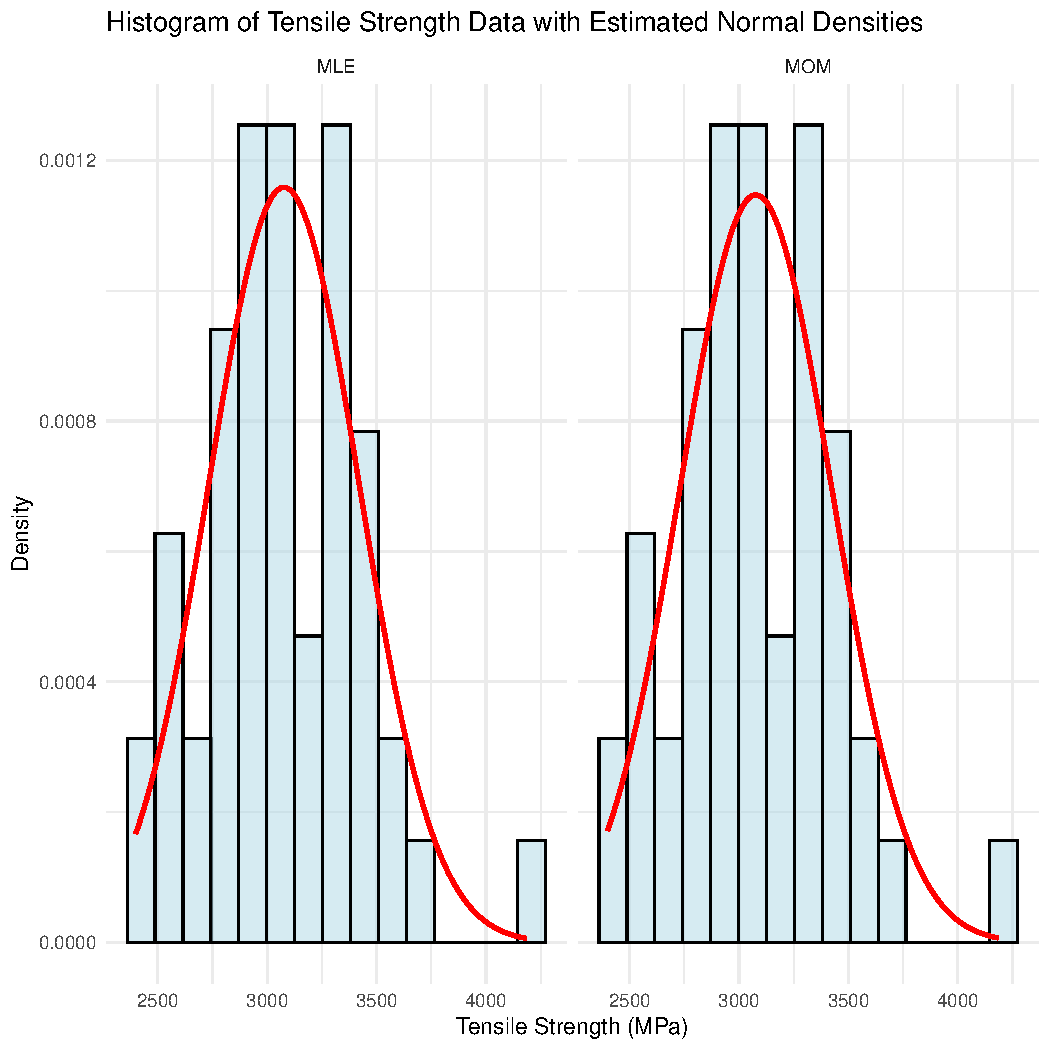
\includegraphics[width=\maxwidth]{figure/unnamed-chunk-1-1} 
\end{knitrout}

\end{document}
